\documentclass{beamer}
\usepackage{listings}\usepackage[utf8]{inputenc}
\usepackage[T1]{fontenc}
\usepackage[french]{babel}
\usepackage{listings}
\usepackage{lmodern}
\usepackage{amsmath}
\usepackage{amssymb}
\usepackage{algorithm}
\usepackage{algpseudocode}
\usepackage{array}
\usepackage{pgf,tikz}
\usepackage{graphicx}
\usepackage{subfig}
%\usepackage{media9}
\usetikzlibrary{arrows}


\usetheme{Warsaw}
\title[]{Réseaux de neurones récurrents et LSTM}
\author[Projet long LSTM]{{\footnotesize Maxime Amossé, Vincent Auriau, Laurent Beaughon, Marc Bélicard, Yaqine Héchaïchi, Julien Hemery, Hugo Hervieux, Sylvain Pascou, \newline Thaïs Rahoul, Pierre Vigier \newline encadrés par Arpad Rimmel et Joanna Tomasik}}
\institute{
\includegraphics[scale=0.3]{images/centralesupelec.jpeg}}
\date{7 juin 2017}

\expandafter\def\expandafter\insertshorttitle\expandafter{%
  \insertshorttitle\hfill%
  \insertframenumber\,/\,\inserttotalframenumber}

\AtBeginSection[]{
  \begin{frame}
  \vfill
  \centering
  \begin{beamercolorbox}[sep=8pt,center,shadow=true,rounded=true]{title}
    \usebeamerfont{title}\insertsectionhead\par%
  \end{beamercolorbox}
  \vfill
  \end{frame}
}

\AtBeginSubsection[]{
  \begin{frame}
  \vfill
  \centering
    \usebeamerfont{title}\insertsubsectionhead\par%
  \vfill
  \end{frame}
}

\setbeamertemplate{headline}{}

\begin{document}

\begin{frame}
\titlepage
\end{frame}

\begin{frame}
\tableofcontents
\end{frame}

\section{Introduction}

\begin{frame}{Objectifs du projet}
  \begin{itemize}
    \item<1-> Étudier les publications originelles
    \item<2-> Implémenter un réseau simple
    \item<3-> Étudier les algorithmes de traitement de séquence
    \item<4-> Implémenter ces algorithmes
    \item<5-> Découvrir la cellule LSTM et l'implémenter
  \end{itemize}
\end{frame}

\section{Ressources}

\begin{frame}{Organisation}
  \begin{itemize}
    \item Réunion hebdomadaire
    \item Suivi des encadrants
    \item Répartition des tâches
  \end{itemize}
\end{frame}

\begin{frame}{Languages et outils}
  \begin{itemize}
    \item Python et Numpy, C++ et Eigen
    \item Github et TravisCI
    \item Zotero
    \item LaTeX
  \end{itemize}
\end{frame}

\section{Principes généraux des réseaux de neurones}

\begin{frame}{Réseau de neurones}
  \begin{figure}
  \begin{center}
  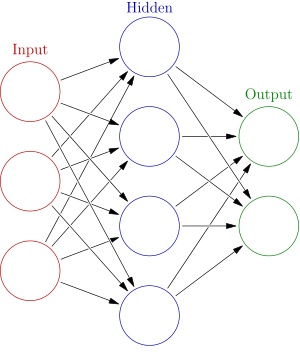
\includegraphics[scale=0.55]{images/reseau_simple.png}
  \caption{Exemple de réseau simple}
  \end{center}
  \end{figure}
\end{frame}

\begin{frame}{Propagation}
  \begin{figure}
  \begin{center}
  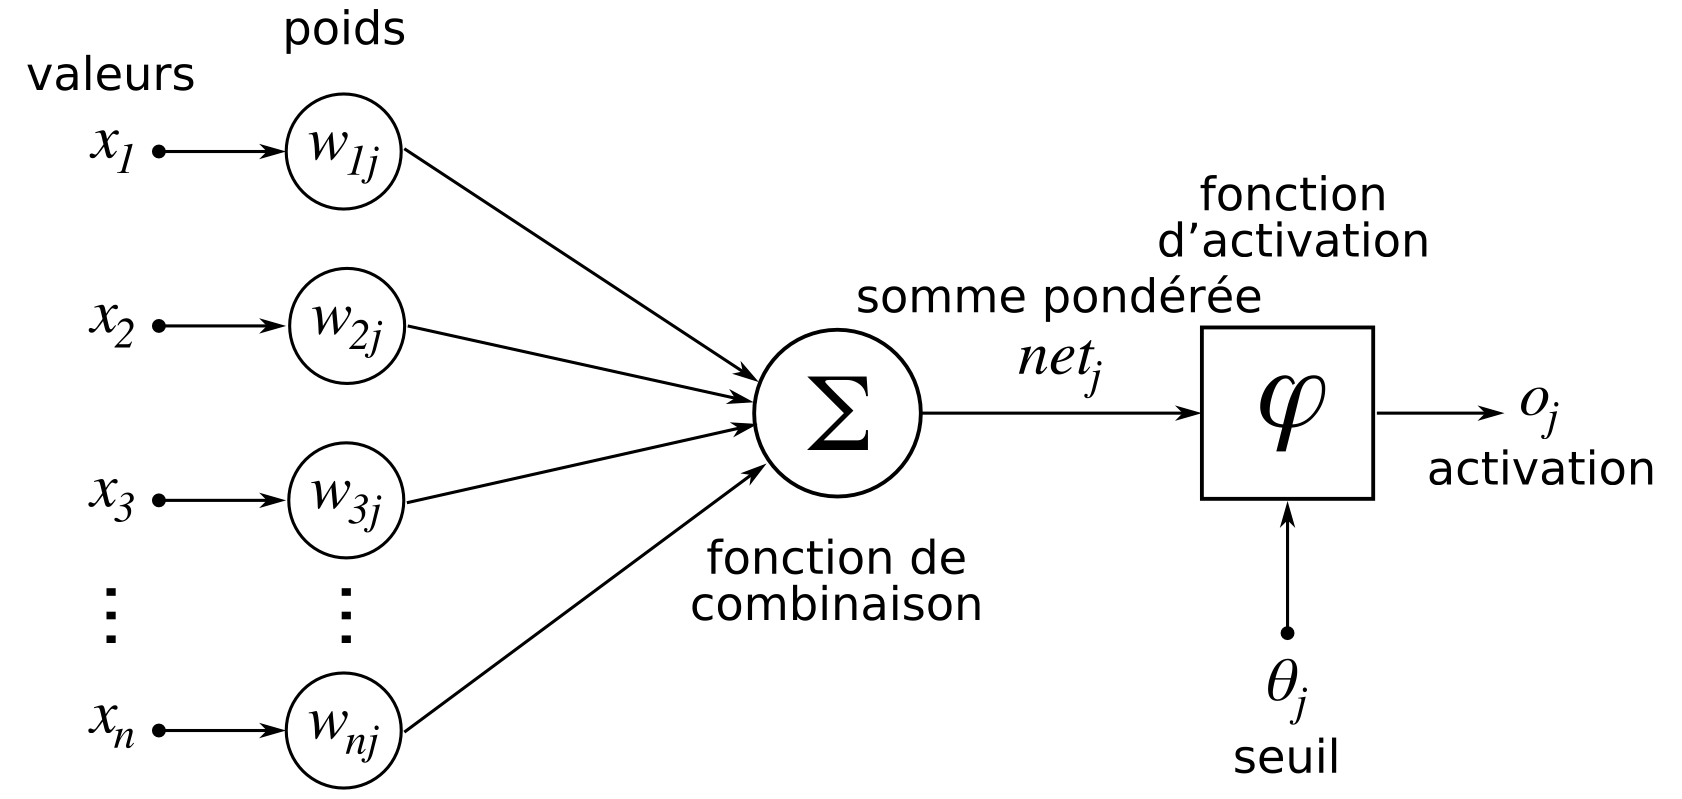
\includegraphics[scale=0.20]{images/propagation_simple.png}
  \caption{Propagation dans une cellule simple}
  {\tiny Source: Wikipedia.org}
  \end{center}
  \end{figure}
\end{frame}

\begin{frame}{Méthode du gradient}
  \begin{figure}
  \begin{center}
  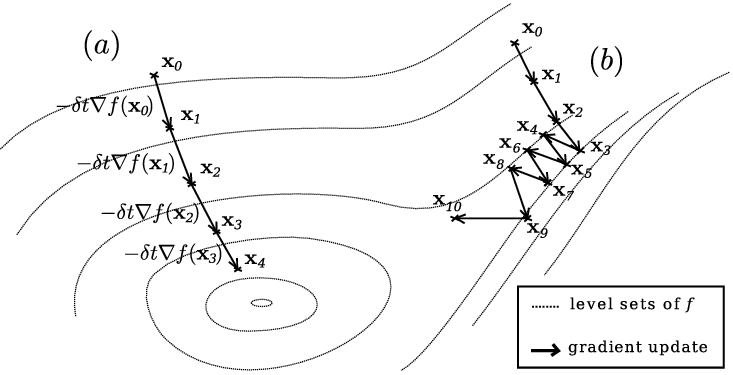
\includegraphics[scale=0.45]{images/descente_gradient.png}
  \caption{Exemples de descente du gradient}
  {\tiny Source: http://ludovicarnold.altervista.org/teaching/optimization/gradient-descent/}
  \end{center}
  \end{figure}
\end{frame}

\begin{frame}{Rétropropagation}
  L'objectif est d'évaluer pour tout $w_{ij}^{(k)}$ :
   $\cfrac{\partial E}{\partial w_{ij}^{(k)}}$.

  \begin{align*}
  \cfrac{\partial E}{\partial w_{ij}^{(k)}} &= \sum_{l = 1}^{M} \cfrac{\partial y_l^{(K)}}{\partial w_{ij}^{(k)}} \times \cfrac{\partial E}{\partial y_l}\\
  \end{align*}

\end{frame}

\begin{frame}{Problème type : MNIST}
  \begin{figure}
  \begin{center}
  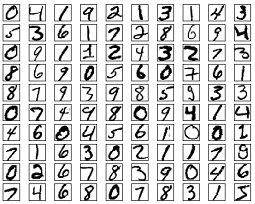
\includegraphics[scale=1.1]{images/mnist_data.png}
  \caption{Exemple de données du MNIST}
  \end{center}
  \end{figure}
\end{frame}

\section{Traitement de séquences, introduction aux réseaux récurrents}

\begin{frame}{Réseau récurrent}
  \begin{figure}
  \begin{center}
  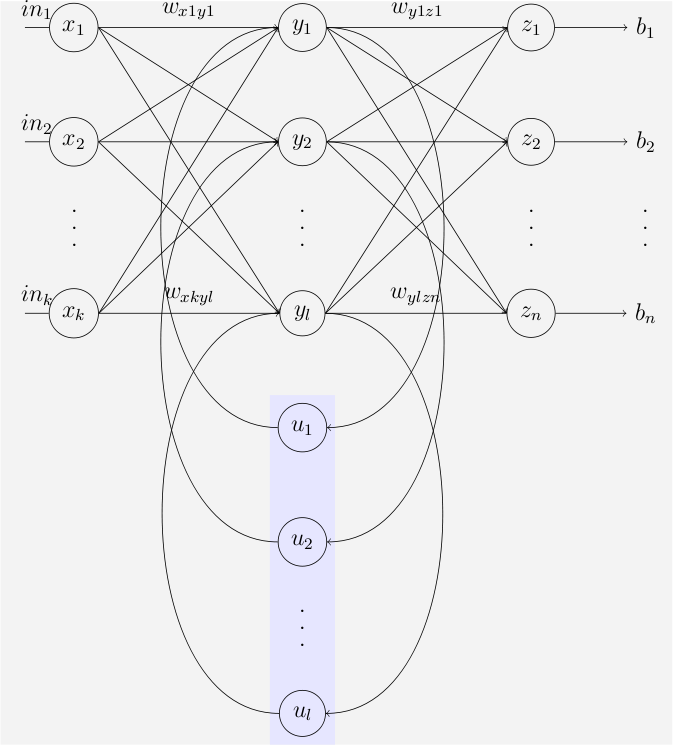
\includegraphics[scale=0.25]{images/reseau_recurrent.png}
  \caption{Exemple de réseau récurrent}
  {\tiny Source: Wikipedia.org}
  \end{center}
  \end{figure}
\end{frame}

\begin{frame}{BPTT}
  \begin{figure}
  \begin{center}
  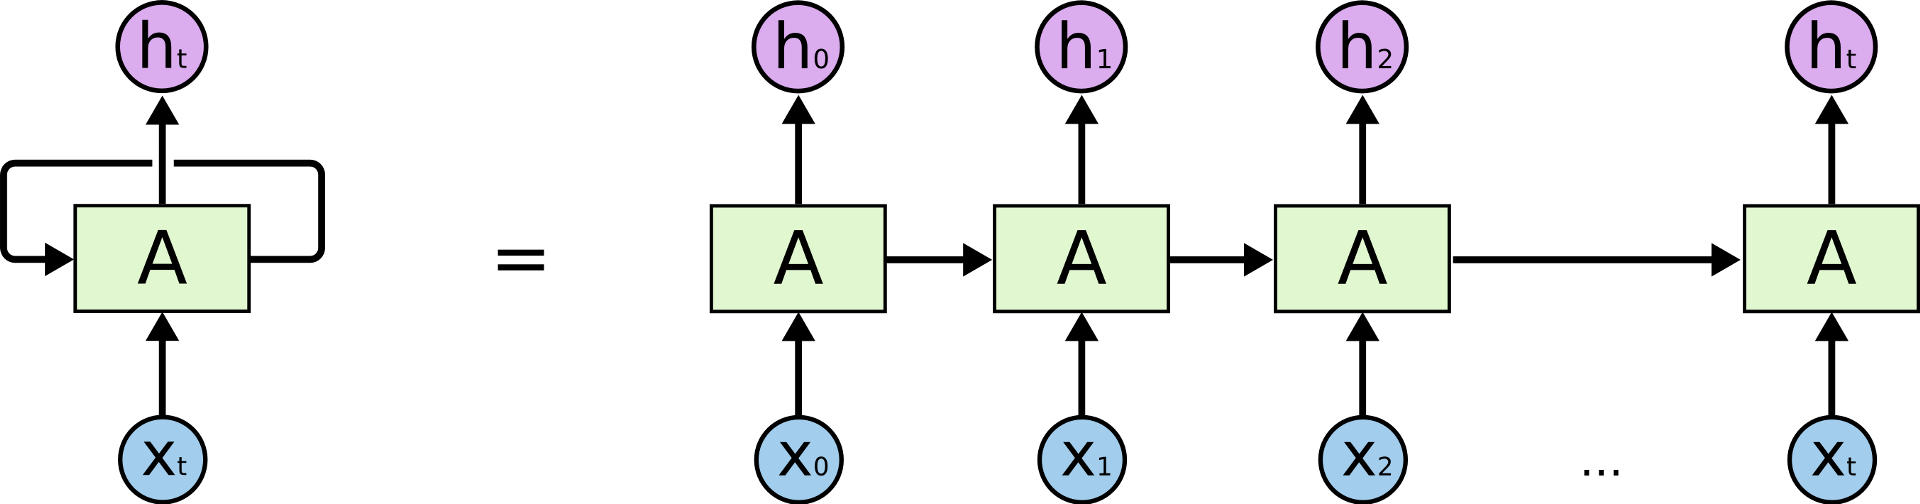
\includegraphics[scale=0.16]{images/bptt.png}
  \caption{Dépliement dans l'espace}
  {\tiny Source: https://colah.github.io/posts/2015-08-Understanding-LSTMs/}
  \end{center}
  \end{figure}
\end{frame}

\begin{frame}{LSTM}
  \begin{figure}
  \begin{center}
  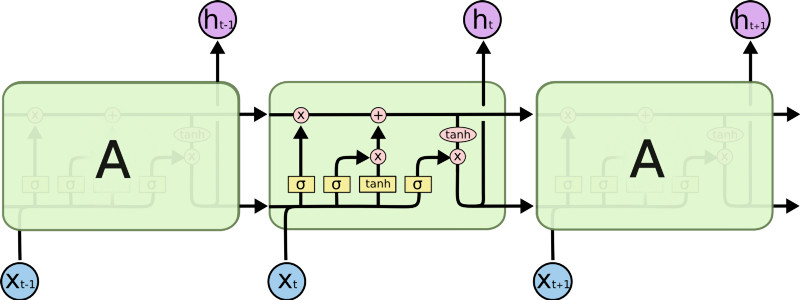
\includegraphics[scale=.40]{images/lstm_bptt.png}
  \caption{Dépliement dans l'espace d'une cellule LSTM}
  {\tiny Source: https://colah.github.io/posts/2015-08-Understanding-LSTMs/}
  \end{center}
  \end{figure}
\end{frame}

\begin{frame}{Comparaison différentes méthodes sur Reber symétrique}
  \begin{figure}
  \begin{center}
  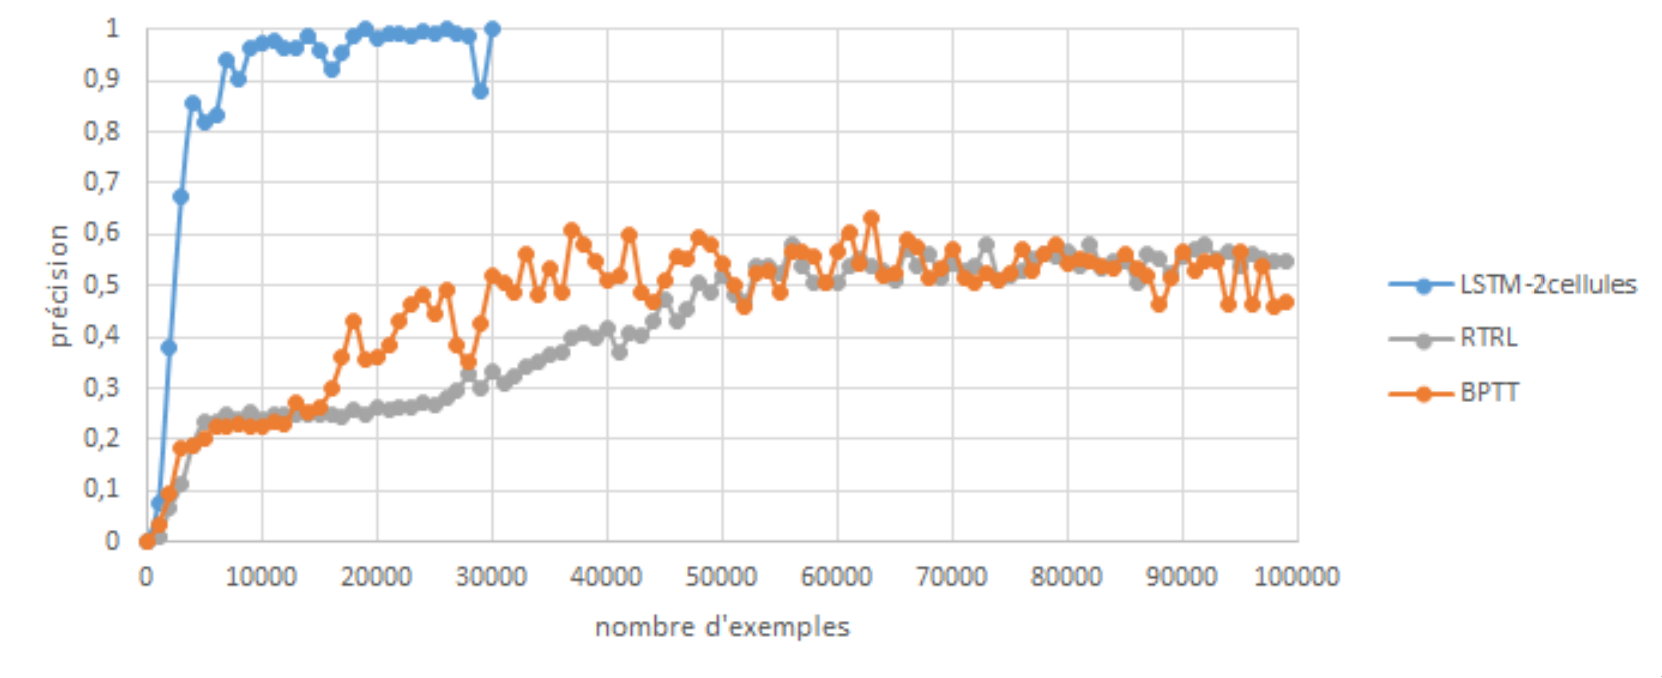
\includegraphics[scale=.20]{images/comparaison.png}
  \caption{Précision de différents algorithmes sur un apprentissage de grammaire de Reber
  symétrique}
  \end{center}
  \end{figure}
\end{frame}

\section{Génération de séquences avec des LSTM}

\begin{frame}{Principe}
\begin{figure}
\begin{center}
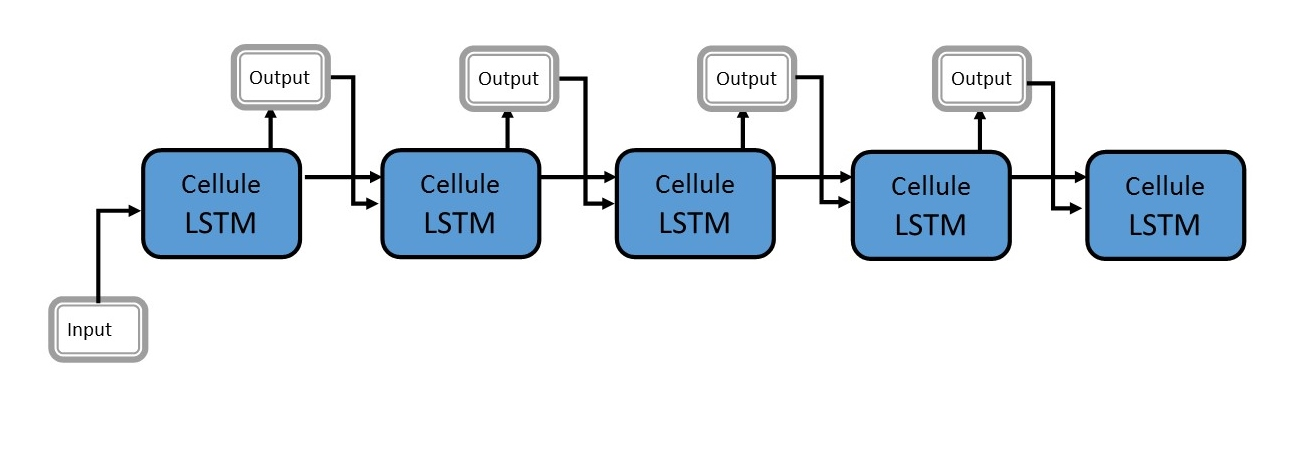
\includegraphics[scale=0.5]{images/lstm_generation.png}
\caption{Principe de génération de séquences}
\end{center}
\end{figure}
\end{frame}


\begin{frame}{Exemple : génération de texte}
Third Servan:\\
Of many bald with him fire, read now?\\
\medbreak
Second Murderer:\\
Out! where he wal’d apt thou, myself!\\
O brother’s maliss and trunks and Caubble subject.\\
Now i’ the fill in thy noble devart wagains to argon me
thy commanded?\\
\medbreak
LADY ANNE:\\
Sir, af you have fellow’s their eyes live?
\end{frame}

\section{Génération de musique}

\begin{frame}{Trois approches différentes}
\begin{figure}
\begin{center}
\begin{tabular}{|c|c|c|c|}
\hline
\textbf{Génération} & \textbf{de spectres} & \textbf{MIDI} & \textbf{de partitions} \\
\hline
Pas de temps & Libres & Libres & Contraints \\
\hline
Hauteurs & Libres & Contraintes & Contraintes \\
\hline
\end{tabular}
\caption{Comparaison des trois approches}
\end{center}
\end{figure}
\end{frame}

\subsection{Génération de spectres audio}

\begin{frame}{Mise en forme des données}
\begin{figure}
\begin{center}
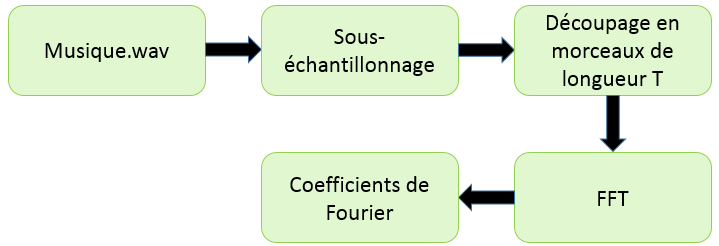
\includegraphics[scale = 0.57]{images/pipeline.png}
\caption{Création du dataset}
\end{center}
\end{figure}
\end{frame}

\begin{frame}{Principe}
\begin{figure}
\begin{center}
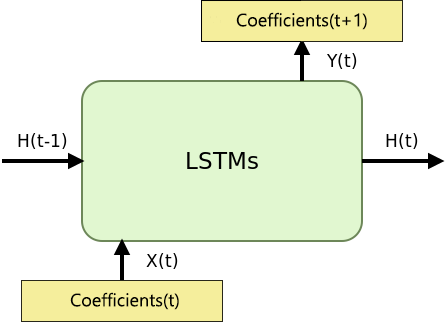
\includegraphics[scale=0.5]{images/fourier.png}
\caption{Fourier RNN}
\end{center}
\end{figure}
\end{frame}

\begin{frame}{Résultats}
\begin{figure}
\begin{center}
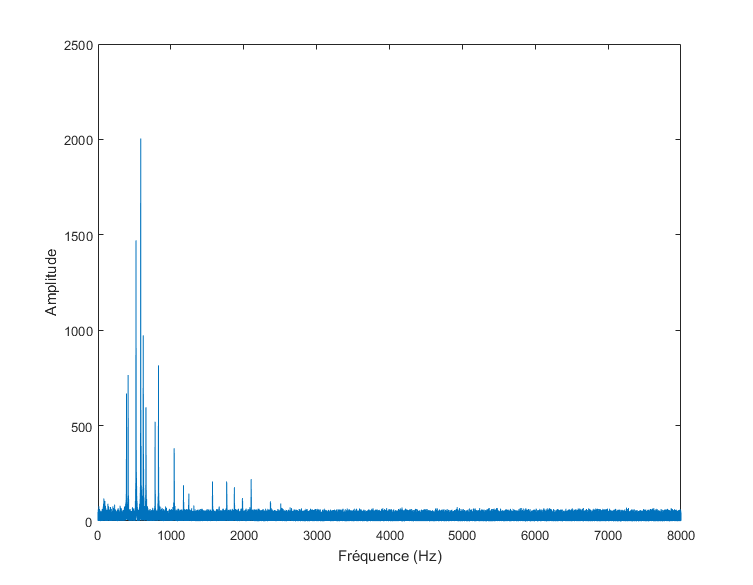
\includegraphics[scale=0.4]{images/spectre.png}
\caption{Spectre du signal généré}
\end{center}
\end{figure}
\end{frame}

\subsection{Génération de midi}

\begin{frame}{Format}
\begin{tiny}
\begin{center}
\begin{tabular}{|c|c|c|c|c|c|c|c|c|c|c|c|c|}
\hline
 & \multicolumn{12}{c|}{\textbf{Hauteurs}} \\
\hline
\textbf{Octave Number} & C & C\# & D & D\# & E & F & F\# & G & G\# & A & A\# & B  \\
\hline
0 & 0 & 1 & 2 & 3 & 4 & 5 & 6 & 7 & 8 & 9 & 10 & 11  \\
\hline
1 & 12 & 13 & 14 & 15 & 16 & 17 & 18 & 19 & 20 & 21 & 22 & 23  \\
\hline
2 & 24 & 25 & 26 & 27 & 28 & 29 & 30 & 31 & 32 & 33 & 34 & 35  \\
\hline
3 & 36 & 37 & 38 & 39 & 40 & 41 & 42 & 43 & 44 & 45 & 46 & 47  \\
\hline
4 & 48 & 49 & 50 & 51 & 52 & 53 & 54 & 55 & 56 & 57 & 58 & 59  \\
\hline
5 & 60 & 61 & 62 & 63 & 64 & 65 & 66 & 67 & 68 & 69 & 70 & 71  \\
\hline
6 & 72 & 73 & 74 & 75 & 76 & 77 & 78 & 79 & 80 & 81 & 82 & 83  \\
\hline
7 & 84 & 85 & 86 & 87 & 88 & 89 & 90 & 91 & 92 & 93 & 94 & 95  \\
\hline
8 & 96 & 97 & 98 & 99 & 100 & 101 & 102 & 103 & 104 & 105 & 106 & 107  \\
\hline
9 & 108 & 109 & 110 & 111 & 112 & 113 & 114 & 115 & 116 & 117 & 118 & 119  \\
\hline
10 & 120 & 121 & 122 & 123 & 124 & 125 & 126 & 127 &   &   &   & \\
\hline
\end{tabular}
\end{center}
\end{tiny}
Commandes :
\begin{itemize}
\item $note\_on \ note \ velocity \ time$
\item $note\_off \ note \ velocity \ time$
\end{itemize}
\end{frame}

\begin{frame}{Principe}
\begin{figure}[!tbp]
  \centering
  \subfloat[Jig]{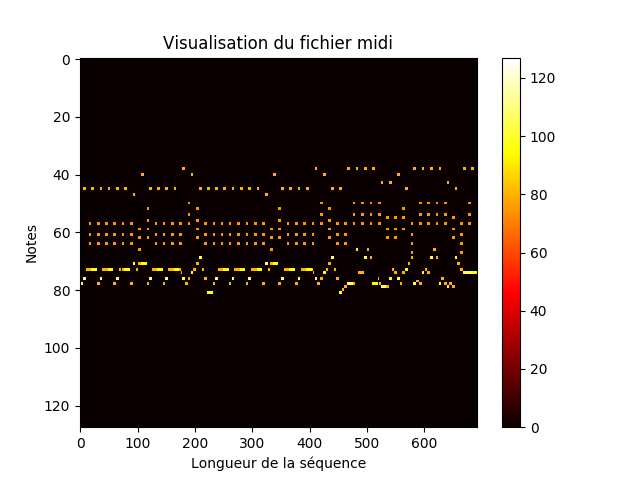
\includegraphics[width=0.5\textwidth]{images/jig1.png}\label{jig}}
  \hfill
  \subfloat[Mozart]{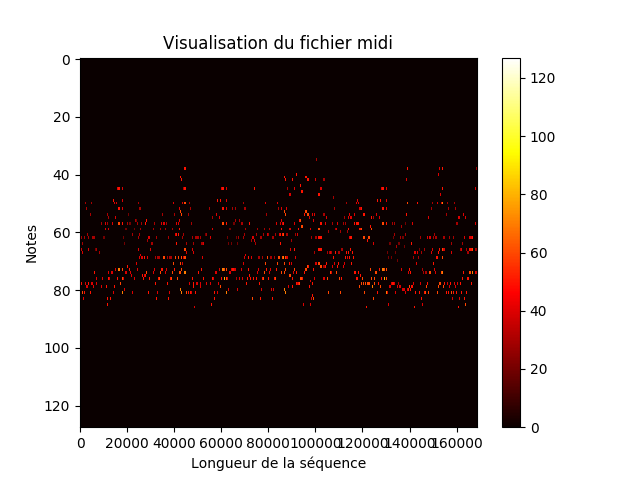
\includegraphics[width=0.5\textwidth]{images/mozart.png}\label{mozart}}
  \caption{Visualisation de fichiers midi}
\end{figure}
\end{frame}

\begin{frame}{Résultats}

\begin{figure}
\begin{center}
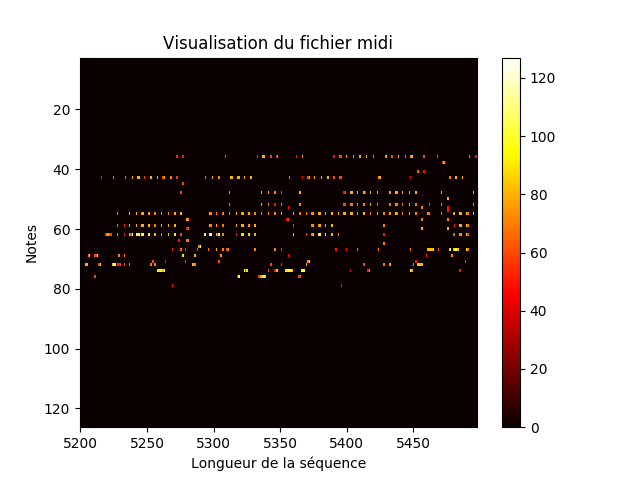
\includegraphics[width=0.5\linewidth]{images/jig_generated_38800.png}
\caption{Jig générée}
\end{center}
\end{figure}
\end{frame}

\subsection{Génération de partitions}

\begin{frame}{Génération de notes}
\begin{figure}
\begin{center}
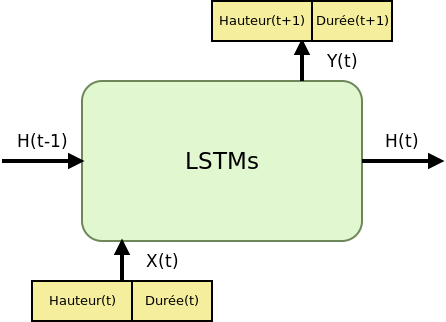
\includegraphics[scale=0.5]{images/note_rnn.png}
\caption{Note RNN}
\end{center}
\end{figure}
\end{frame}

\begin{frame}{Résultats}
\begin{figure}
\begin{center}
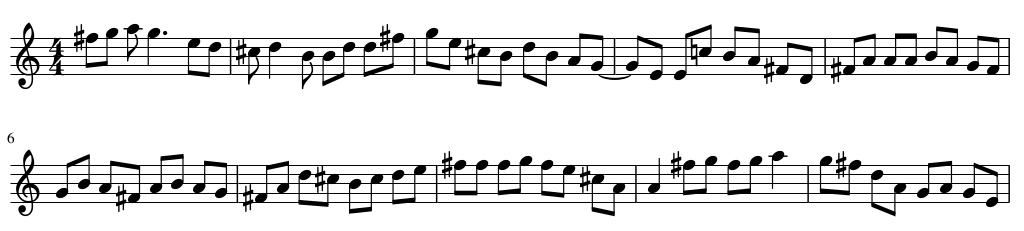
\includegraphics[scale=0.3]{images/note_rnn_result.png}
\caption{Une partition générée par Note RNN}
\end{center}
\end{figure}
\end{frame}

\begin{frame}{Génération de notes en série}
\begin{figure}
\begin{center}
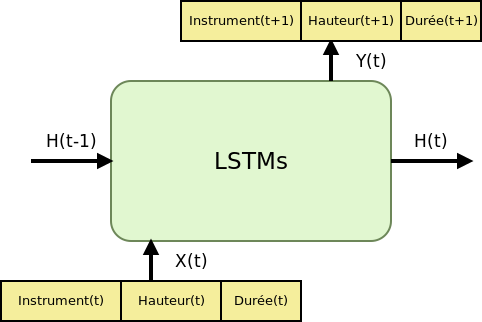
\includegraphics[scale=0.5]{images/series_rnn.png}
\caption{Series RNN}
\end{center}
\end{figure}
\end{frame}

\begin{frame}{Résultats}
\begin{figure}
\begin{center}
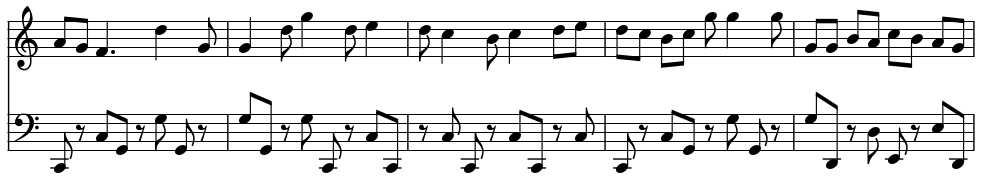
\includegraphics[scale=0.3]{images/series_rnn_result.png}
\caption{Une partition générée par Series RNN}
\end{center}
\end{figure}
\end{frame}

\begin{frame}{Génération de mesures en parallèle}
\begin{figure}
\begin{center}
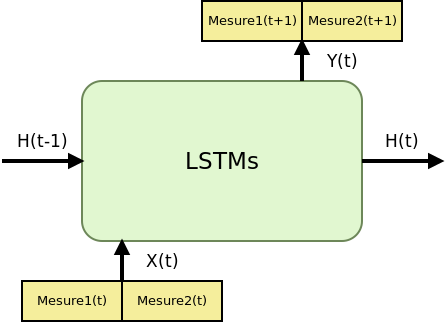
\includegraphics[scale=0.5]{images/measure_rnn.png}
\caption{Measure RNN}
\end{center}
\end{figure}
\end{frame}

\begin{frame}{Encodage des mesures}
\begin{figure}
\begin{center}
% Graphic for TeX using PGF
% Title: /home/pierre/Programming/pl-lstm/images/illustrations_cr/autoencoder.dia
% Creator: Dia v0.97.3
% CreationDate: Fri May 19 11:26:39 2017
% For: pierre
% \usepackage{tikz}
% The following commands are not supported in PSTricks at present
% We define them conditionally, so when they are implemented,
% this pgf file will use them.
\ifx\du\undefined
  \newlength{\du}
\fi
\setlength{\du}{15\unitlength}
\begin{tikzpicture}[scale=0.6]
\pgftransformxscale{1.000000}
\pgftransformyscale{-1.000000}
\definecolor{dialinecolor}{rgb}{0.000000, 0.000000, 0.000000}
\pgfsetstrokecolor{dialinecolor}
\definecolor{dialinecolor}{rgb}{1.000000, 1.000000, 1.000000}
\pgfsetfillcolor{dialinecolor}
\pgfsetlinewidth{0.050000\du}
\pgfsetdash{}{0pt}
\pgfsetdash{}{0pt}
\pgfsetmiterjoin
\definecolor{dialinecolor}{rgb}{1.000000, 1.000000, 1.000000}
\pgfsetfillcolor{dialinecolor}
\fill (12.000000\du,13.000000\du)--(12.000000\du,15.000000\du)--(15.000000\du,15.000000\du)--(15.000000\du,13.000000\du)--cycle;
\definecolor{dialinecolor}{rgb}{0.000000, 0.000000, 0.000000}
\pgfsetstrokecolor{dialinecolor}
\draw (12.000000\du,13.000000\du)--(12.000000\du,15.000000\du)--(15.000000\du,15.000000\du)--(15.000000\du,13.000000\du)--cycle;
\pgfsetlinewidth{0.050000\du}
\pgfsetdash{}{0pt}
\pgfsetdash{}{0pt}
\pgfsetmiterjoin
\definecolor{dialinecolor}{rgb}{1.000000, 1.000000, 1.000000}
\pgfsetfillcolor{dialinecolor}
\fill (17.000000\du,13.000000\du)--(17.000000\du,15.000000\du)--(20.000000\du,15.000000\du)--(20.000000\du,13.000000\du)--cycle;
\definecolor{dialinecolor}{rgb}{0.000000, 0.000000, 0.000000}
\pgfsetstrokecolor{dialinecolor}
\draw (17.000000\du,13.000000\du)--(17.000000\du,15.000000\du)--(20.000000\du,15.000000\du)--(20.000000\du,13.000000\du)--cycle;
\pgfsetlinewidth{0.050000\du}
\pgfsetdash{}{0pt}
\pgfsetdash{}{0pt}
\pgfsetmiterjoin
\definecolor{dialinecolor}{rgb}{1.000000, 1.000000, 1.000000}
\pgfsetfillcolor{dialinecolor}
\fill (27.000000\du,13.000000\du)--(27.000000\du,15.000000\du)--(30.000000\du,15.000000\du)--(30.000000\du,13.000000\du)--cycle;
\definecolor{dialinecolor}{rgb}{0.000000, 0.000000, 0.000000}
\pgfsetstrokecolor{dialinecolor}
\draw (27.000000\du,13.000000\du)--(27.000000\du,15.000000\du)--(30.000000\du,15.000000\du)--(30.000000\du,13.000000\du)--cycle;
\pgfsetlinewidth{0.050000\du}
\pgfsetdash{}{0pt}
\pgfsetdash{}{0pt}
\pgfsetmiterjoin
\definecolor{dialinecolor}{rgb}{1.000000, 1.000000, 1.000000}
\pgfsetfillcolor{dialinecolor}
\fill (32.000000\du,13.000000\du)--(32.000000\du,15.000000\du)--(35.000000\du,15.000000\du)--(35.000000\du,13.000000\du)--cycle;
\definecolor{dialinecolor}{rgb}{0.000000, 0.000000, 0.000000}
\pgfsetstrokecolor{dialinecolor}
\draw (32.000000\du,13.000000\du)--(32.000000\du,15.000000\du)--(35.000000\du,15.000000\du)--(35.000000\du,13.000000\du)--cycle;
\pgfsetlinewidth{0.050000\du}
\pgfsetdash{}{0pt}
\pgfsetdash{}{0pt}
\pgfsetmiterjoin
\pgfsetbuttcap
{
\definecolor{dialinecolor}{rgb}{0.000000, 0.000000, 0.000000}
\pgfsetfillcolor{dialinecolor}
% was here!!!
\pgfsetarrowsend{latex}
{\pgfsetcornersarced{\pgfpoint{0.000000\du}{0.000000\du}}\definecolor{dialinecolor}{rgb}{0.000000, 0.000000, 0.000000}
\pgfsetstrokecolor{dialinecolor}
\draw (37.000000\du,10.000000\du)--(37.000000\du,9.000000\du)--(34.000000\du,9.000000\du)--(34.000000\du,8.000000\du);
}}
\pgfsetlinewidth{0.050000\du}
\pgfsetdash{}{0pt}
\pgfsetdash{}{0pt}
\pgfsetmiterjoin
\definecolor{dialinecolor}{rgb}{1.000000, 1.000000, 1.000000}
\pgfsetfillcolor{dialinecolor}
\fill (12.000000\du,6.000000\du)--(12.000000\du,8.000000\du)--(15.000000\du,8.000000\du)--(15.000000\du,6.000000\du)--cycle;
\definecolor{dialinecolor}{rgb}{0.000000, 0.000000, 0.000000}
\pgfsetstrokecolor{dialinecolor}
\draw (12.000000\du,6.000000\du)--(12.000000\du,8.000000\du)--(15.000000\du,8.000000\du)--(15.000000\du,6.000000\du)--cycle;
\pgfsetlinewidth{0.050000\du}
\pgfsetdash{}{0pt}
\pgfsetdash{}{0pt}
\pgfsetmiterjoin
\definecolor{dialinecolor}{rgb}{1.000000, 1.000000, 1.000000}
\pgfsetfillcolor{dialinecolor}
\fill (17.000000\du,6.000000\du)--(17.000000\du,8.000000\du)--(20.000000\du,8.000000\du)--(20.000000\du,6.000000\du)--cycle;
\definecolor{dialinecolor}{rgb}{0.000000, 0.000000, 0.000000}
\pgfsetstrokecolor{dialinecolor}
\draw (17.000000\du,6.000000\du)--(17.000000\du,8.000000\du)--(20.000000\du,8.000000\du)--(20.000000\du,6.000000\du)--cycle;
\pgfsetlinewidth{0.050000\du}
\pgfsetdash{}{0pt}
\pgfsetdash{}{0pt}
\pgfsetmiterjoin
\definecolor{dialinecolor}{rgb}{1.000000, 1.000000, 1.000000}
\pgfsetfillcolor{dialinecolor}
\fill (27.000000\du,6.000000\du)--(27.000000\du,8.000000\du)--(30.000000\du,8.000000\du)--(30.000000\du,6.000000\du)--cycle;
\definecolor{dialinecolor}{rgb}{0.000000, 0.000000, 0.000000}
\pgfsetstrokecolor{dialinecolor}
\draw (27.000000\du,6.000000\du)--(27.000000\du,8.000000\du)--(30.000000\du,8.000000\du)--(30.000000\du,6.000000\du)--cycle;
\pgfsetlinewidth{0.050000\du}
\pgfsetdash{}{0pt}
\pgfsetdash{}{0pt}
\pgfsetmiterjoin
\definecolor{dialinecolor}{rgb}{1.000000, 1.000000, 1.000000}
\pgfsetfillcolor{dialinecolor}
\fill (32.000000\du,6.000000\du)--(32.000000\du,8.000000\du)--(35.000000\du,8.000000\du)--(35.000000\du,6.000000\du)--cycle;
\definecolor{dialinecolor}{rgb}{0.000000, 0.000000, 0.000000}
\pgfsetstrokecolor{dialinecolor}
\draw (32.000000\du,6.000000\du)--(32.000000\du,8.000000\du)--(35.000000\du,8.000000\du)--(35.000000\du,6.000000\du)--cycle;
\pgfsetlinewidth{0.050000\du}
\pgfsetdash{}{0pt}
\pgfsetdash{}{0pt}
\pgfsetbuttcap
{
\definecolor{dialinecolor}{rgb}{0.000000, 0.000000, 0.000000}
\pgfsetfillcolor{dialinecolor}
% was here!!!
\pgfsetarrowsend{latex}
\definecolor{dialinecolor}{rgb}{0.000000, 0.000000, 0.000000}
\pgfsetstrokecolor{dialinecolor}
\draw (13.000000\du,16.000000\du)--(13.000000\du,15.000000\du);
}
\pgfsetlinewidth{0.050000\du}
\pgfsetdash{}{0pt}
\pgfsetdash{}{0pt}
\pgfsetbuttcap
{
\definecolor{dialinecolor}{rgb}{0.000000, 0.000000, 0.000000}
\pgfsetfillcolor{dialinecolor}
% was here!!!
\pgfsetarrowsend{latex}
\definecolor{dialinecolor}{rgb}{0.000000, 0.000000, 0.000000}
\pgfsetstrokecolor{dialinecolor}
\draw (18.000000\du,16.000000\du)--(18.000000\du,15.000000\du);
}
\pgfsetlinewidth{0.050000\du}
\pgfsetdash{}{0pt}
\pgfsetdash{}{0pt}
\pgfsetbuttcap
{
\definecolor{dialinecolor}{rgb}{0.000000, 0.000000, 0.000000}
\pgfsetfillcolor{dialinecolor}
% was here!!!
\pgfsetarrowsend{latex}
\definecolor{dialinecolor}{rgb}{0.000000, 0.000000, 0.000000}
\pgfsetstrokecolor{dialinecolor}
\draw (28.000000\du,16.000000\du)--(28.000000\du,15.000000\du);
}
\pgfsetlinewidth{0.050000\du}
\pgfsetdash{}{0pt}
\pgfsetdash{}{0pt}
\pgfsetbuttcap
{
\definecolor{dialinecolor}{rgb}{0.000000, 0.000000, 0.000000}
\pgfsetfillcolor{dialinecolor}
% was here!!!
\pgfsetarrowsend{latex}
\definecolor{dialinecolor}{rgb}{0.000000, 0.000000, 0.000000}
\pgfsetstrokecolor{dialinecolor}
\draw (33.000000\du,16.000000\du)--(33.000000\du,15.000000\du);
}
\pgfsetlinewidth{0.050000\du}
\pgfsetdash{}{0pt}
\pgfsetdash{}{0pt}
\pgfsetbuttcap
{
\definecolor{dialinecolor}{rgb}{0.000000, 0.000000, 0.000000}
\pgfsetfillcolor{dialinecolor}
% was here!!!
\pgfsetarrowsend{latex}
\definecolor{dialinecolor}{rgb}{0.000000, 0.000000, 0.000000}
\pgfsetstrokecolor{dialinecolor}
\draw (32.000000\du,7.000000\du)--(30.000000\du,7.000000\du);
}
\pgfsetlinewidth{0.050000\du}
\pgfsetdash{}{0pt}
\pgfsetdash{}{0pt}
\pgfsetbuttcap
{
\definecolor{dialinecolor}{rgb}{0.000000, 0.000000, 0.000000}
\pgfsetfillcolor{dialinecolor}
% was here!!!
\pgfsetarrowsend{latex}
\definecolor{dialinecolor}{rgb}{0.000000, 0.000000, 0.000000}
\pgfsetstrokecolor{dialinecolor}
\draw (27.000000\du,7.000000\du)--(25.000000\du,7.000000\du);
}
\pgfsetlinewidth{0.050000\du}
\pgfsetdash{}{0pt}
\pgfsetdash{}{0pt}
\pgfsetbuttcap
{
\definecolor{dialinecolor}{rgb}{0.000000, 0.000000, 0.000000}
\pgfsetfillcolor{dialinecolor}
% was here!!!
\pgfsetarrowsend{latex}
\definecolor{dialinecolor}{rgb}{0.000000, 0.000000, 0.000000}
\pgfsetstrokecolor{dialinecolor}
\draw (17.000000\du,7.000000\du)--(15.000000\du,7.000000\du);
}
\pgfsetlinewidth{0.050000\du}
\pgfsetdash{}{0pt}
\pgfsetdash{}{0pt}
\pgfsetbuttcap
{
\definecolor{dialinecolor}{rgb}{0.000000, 0.000000, 0.000000}
\pgfsetfillcolor{dialinecolor}
% was here!!!
\pgfsetarrowsend{latex}
\definecolor{dialinecolor}{rgb}{0.000000, 0.000000, 0.000000}
\pgfsetstrokecolor{dialinecolor}
\draw (15.000000\du,14.000000\du)--(17.000000\du,14.000000\du);
}
\pgfsetlinewidth{0.050000\du}
\pgfsetdash{}{0pt}
\pgfsetdash{}{0pt}
\pgfsetbuttcap
{
\definecolor{dialinecolor}{rgb}{0.000000, 0.000000, 0.000000}
\pgfsetfillcolor{dialinecolor}
% was here!!!
\pgfsetarrowsend{latex}
\definecolor{dialinecolor}{rgb}{0.000000, 0.000000, 0.000000}
\pgfsetstrokecolor{dialinecolor}
\draw (20.000000\du,14.000000\du)--(22.000000\du,14.000000\du);
}
\pgfsetlinewidth{0.050000\du}
\pgfsetdash{}{0pt}
\pgfsetdash{}{0pt}
\pgfsetbuttcap
{
\definecolor{dialinecolor}{rgb}{0.000000, 0.000000, 0.000000}
\pgfsetfillcolor{dialinecolor}
% was here!!!
\pgfsetarrowsend{latex}
\definecolor{dialinecolor}{rgb}{0.000000, 0.000000, 0.000000}
\pgfsetstrokecolor{dialinecolor}
\draw (30.000000\du,14.000000\du)--(32.000000\du,14.000000\du);
}
% setfont left to latex
\definecolor{dialinecolor}{rgb}{0.000000, 0.000000, 0.000000}
\pgfsetstrokecolor{dialinecolor}
\node at (37.000000\du,11.293750\du){$c$};
% setfont left to latex
\definecolor{dialinecolor}{rgb}{0.000000, 0.000000, 0.000000}
\pgfsetstrokecolor{dialinecolor}
\node at (13.000000\du,17.293750\du){$x_1$};
\pgfsetlinewidth{0.050000\du}
\pgfsetdash{}{0pt}
\pgfsetdash{}{0pt}
\pgfsetbuttcap
{
\definecolor{dialinecolor}{rgb}{0.000000, 0.000000, 0.000000}
\pgfsetfillcolor{dialinecolor}
% was here!!!
\pgfsetarrowsend{latex}
\definecolor{dialinecolor}{rgb}{0.000000, 0.000000, 0.000000}
\pgfsetstrokecolor{dialinecolor}
\draw (25.000000\du,14.000000\du)--(27.000000\du,14.000000\du);
}
\pgfsetlinewidth{0.050000\du}
\pgfsetdash{}{0pt}
\pgfsetdash{}{0pt}
\pgfsetbuttcap
{
\definecolor{dialinecolor}{rgb}{0.000000, 0.000000, 0.000000}
\pgfsetfillcolor{dialinecolor}
% was here!!!
\pgfsetarrowsend{latex}
\definecolor{dialinecolor}{rgb}{0.000000, 0.000000, 0.000000}
\pgfsetstrokecolor{dialinecolor}
\draw (22.000000\du,7.000000\du)--(20.000000\du,7.000000\du);
}
% setfont left to latex
\definecolor{dialinecolor}{rgb}{0.000000, 0.000000, 0.000000}
\pgfsetstrokecolor{dialinecolor}
\node at (23.500000\du,7.293750\du){...};
% setfont left to latex
\definecolor{dialinecolor}{rgb}{0.000000, 0.000000, 0.000000}
\pgfsetstrokecolor{dialinecolor}
\node at (23.500000\du,14.293750\du){...};
% setfont left to latex
\definecolor{dialinecolor}{rgb}{0.000000, 0.000000, 0.000000}
\pgfsetstrokecolor{dialinecolor}
\node at (18.000000\du,17.293750\du){$x_2$};
% setfont left to latex
\definecolor{dialinecolor}{rgb}{0.000000, 0.000000, 0.000000}
\pgfsetstrokecolor{dialinecolor}
\node at (28.000000\du,17.293750\du){$x_M$};
% setfont left to latex
\definecolor{dialinecolor}{rgb}{0.000000, 0.000000, 0.000000}
\pgfsetstrokecolor{dialinecolor}
\node at (33.000000\du,17.293750\du){<eos>};
\pgfsetlinewidth{0.050000\du}
\pgfsetdash{}{0pt}
\pgfsetdash{}{0pt}
\pgfsetbuttcap
{
\definecolor{dialinecolor}{rgb}{0.000000, 0.000000, 0.000000}
\pgfsetfillcolor{dialinecolor}
% was here!!!
\pgfsetarrowsend{latex}
\definecolor{dialinecolor}{rgb}{0.000000, 0.000000, 0.000000}
\pgfsetstrokecolor{dialinecolor}
\draw (13.000000\du,6.000000\du)--(13.000000\du,5.000000\du);
}
\pgfsetlinewidth{0.050000\du}
\pgfsetdash{}{0pt}
\pgfsetdash{}{0pt}
\pgfsetbuttcap
{
\definecolor{dialinecolor}{rgb}{0.000000, 0.000000, 0.000000}
\pgfsetfillcolor{dialinecolor}
% was here!!!
\pgfsetarrowsend{latex}
\definecolor{dialinecolor}{rgb}{0.000000, 0.000000, 0.000000}
\pgfsetstrokecolor{dialinecolor}
\draw (18.000000\du,6.000000\du)--(18.000000\du,5.000000\du);
}
\pgfsetlinewidth{0.050000\du}
\pgfsetdash{}{0pt}
\pgfsetdash{}{0pt}
\pgfsetbuttcap
{
\definecolor{dialinecolor}{rgb}{0.000000, 0.000000, 0.000000}
\pgfsetfillcolor{dialinecolor}
% was here!!!
\pgfsetarrowsend{latex}
\definecolor{dialinecolor}{rgb}{0.000000, 0.000000, 0.000000}
\pgfsetstrokecolor{dialinecolor}
\draw (28.000000\du,6.000000\du)--(28.000000\du,5.000000\du);
}
\pgfsetlinewidth{0.050000\du}
\pgfsetdash{}{0pt}
\pgfsetdash{}{0pt}
\pgfsetbuttcap
{
\definecolor{dialinecolor}{rgb}{0.000000, 0.000000, 0.000000}
\pgfsetfillcolor{dialinecolor}
% was here!!!
\pgfsetarrowsend{latex}
\definecolor{dialinecolor}{rgb}{0.000000, 0.000000, 0.000000}
\pgfsetstrokecolor{dialinecolor}
\draw (33.000000\du,6.000000\du)--(33.000000\du,5.000000\du);
}
% setfont left to latex
\definecolor{dialinecolor}{rgb}{0.000000, 0.000000, 0.000000}
\pgfsetstrokecolor{dialinecolor}
\node at (13.000000\du,4.293750\du){<eos>};
% setfont left to latex
\definecolor{dialinecolor}{rgb}{0.000000, 0.000000, 0.000000}
\pgfsetstrokecolor{dialinecolor}
\node at (18.000000\du,4.293750\du){$\hat{x}_N$};
% setfont left to latex
\definecolor{dialinecolor}{rgb}{0.000000, 0.000000, 0.000000}
\pgfsetstrokecolor{dialinecolor}
\node at (28.000000\du,4.293750\du){$\hat{x}_2$};
% setfont left to latex
\definecolor{dialinecolor}{rgb}{0.000000, 0.000000, 0.000000}
\pgfsetstrokecolor{dialinecolor}
\node at (33.000000\du,4.293750\du){$\hat{x}_1$};
\pgfsetlinewidth{0.050000\du}
\pgfsetdash{}{0pt}
\pgfsetdash{}{0pt}
\pgfsetbuttcap
{
\definecolor{dialinecolor}{rgb}{0.000000, 0.000000, 0.000000}
\pgfsetfillcolor{dialinecolor}
% was here!!!
\pgfsetarrowsend{latex}
\definecolor{dialinecolor}{rgb}{0.000000, 0.000000, 0.000000}
\pgfsetstrokecolor{dialinecolor}
\draw (13.000000\du,9.000000\du)--(13.000000\du,8.000000\du);
}
\pgfsetlinewidth{0.050000\du}
\pgfsetdash{}{0pt}
\pgfsetdash{}{0pt}
\pgfsetbuttcap
{
\definecolor{dialinecolor}{rgb}{0.000000, 0.000000, 0.000000}
\pgfsetfillcolor{dialinecolor}
% was here!!!
\definecolor{dialinecolor}{rgb}{0.000000, 0.000000, 0.000000}
\pgfsetstrokecolor{dialinecolor}
\draw (13.000000\du,9.000000\du)--(34.000000\du,9.000000\du);
}
\pgfsetlinewidth{0.050000\du}
\pgfsetdash{}{0pt}
\pgfsetdash{}{0pt}
\pgfsetbuttcap
{
\definecolor{dialinecolor}{rgb}{0.000000, 0.000000, 0.000000}
\pgfsetfillcolor{dialinecolor}
% was here!!!
\pgfsetarrowsend{latex}
\definecolor{dialinecolor}{rgb}{0.000000, 0.000000, 0.000000}
\pgfsetstrokecolor{dialinecolor}
\draw (18.000000\du,9.000000\du)--(18.000000\du,8.000000\du);
}
\pgfsetlinewidth{0.050000\du}
\pgfsetdash{}{0pt}
\pgfsetdash{}{0pt}
\pgfsetbuttcap
{
\definecolor{dialinecolor}{rgb}{0.000000, 0.000000, 0.000000}
\pgfsetfillcolor{dialinecolor}
% was here!!!
\pgfsetarrowsend{latex}
\definecolor{dialinecolor}{rgb}{0.000000, 0.000000, 0.000000}
\pgfsetstrokecolor{dialinecolor}
\draw (28.000000\du,9.000000\du)--(28.000000\du,8.000000\du);
}
\pgfsetlinewidth{0.050000\du}
\pgfsetdash{}{0pt}
\pgfsetdash{}{0pt}
\pgfsetbuttcap
{
\definecolor{dialinecolor}{rgb}{0.000000, 0.000000, 0.000000}
\pgfsetfillcolor{dialinecolor}
% was here!!!
\definecolor{dialinecolor}{rgb}{0.000000, 0.000000, 0.000000}
\pgfsetstrokecolor{dialinecolor}
\draw (35.000000\du,14.000000\du)--(37.000000\du,14.000000\du);
}
\pgfsetlinewidth{0.050000\du}
\pgfsetdash{}{0pt}
\pgfsetdash{}{0pt}
\pgfsetbuttcap
{
\definecolor{dialinecolor}{rgb}{0.000000, 0.000000, 0.000000}
\pgfsetfillcolor{dialinecolor}
% was here!!!
\pgfsetarrowsend{latex}
\definecolor{dialinecolor}{rgb}{0.000000, 0.000000, 0.000000}
\pgfsetstrokecolor{dialinecolor}
\draw (37.000000\du,14.000000\du)--(37.000000\du,12.000000\du);
}
\end{tikzpicture}

\caption{Réseau encodeur de mesures}
\end{center}
\end{figure}
\end{frame}

\begin{frame}{Résultats}
\begin{figure}
\begin{center}
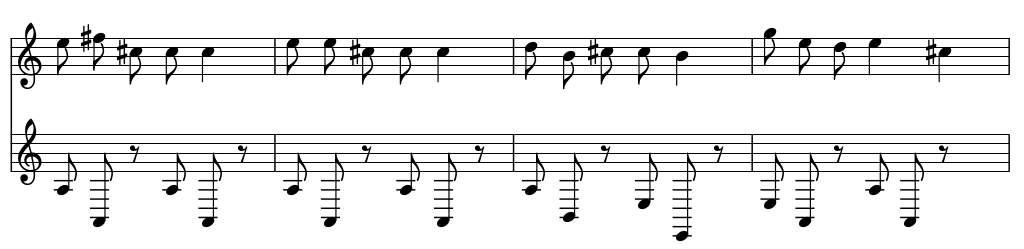
\includegraphics[scale=0.3]{images/measure_rnn_result.png}
\caption{Une partition générée par Measure RNN}
\end{center}
\end{figure}
\end{frame}

\section{Conclusion}
\end{document}
